%
% cwt.tex
%
% (c) 2019 Prof Dr Andreas Müller, Hochschule Rapperswil
%
\section{Stetige Wavelet-Transformation
\label{sextion:cwt}}
\rhead{Stetige Wavelet-Transformation}
Ein Wavelet soll nun dazu verwendet werden, ein Signal $f(t)$
abzutasten.
Da das Wavelet lokalisiert ist, müssen wir es der $t$-Achse entlang
verschieben, um jeden Abschnitt des Signals sinnvoll abtasten zu
können.
Da das Wavelet auch im Frequenzbereich lokalisiert ist, müssen wir
es ausserdem skalieren, um sowohl kurzwellige wie auch langwellige
Details des Signals zu erfassen.

Sei also $\psi$ ein Wavelet, also eine Funktion, die die
Zulässigkeitsbedingung~\eqref{cwt:zulaessig} erfüllt\footnote{Die nachfolgenden
Definitionen sind zum Teil auch sinnvoll, wenn die Zulässigkeitsbedingung
nicht erfüllt ist, doch ist die so entstehende Transformation nicht unbedingt
stetig oder umkehrbar.}.
Wir setzen daher
\[
\psi_{a,b}(t) = \frac{1}{\sqrt{|a|}} \psi\biggl(\frac{t-b}a\biggr).
\]
Den Spezialfall $b=0$ kürzen wir $\psi_a = \psi_{a,0}$ ab.

\begin{lemma}
Die verschobenen und gestreckten Kopien $\psi_{a,b}$ von $\psi$ haben alle
die gleiche Norm: $\|\psi_{a,b}\|=1$.
\end{lemma}

\begin{proof}[Beweis]
Zunächst ist klar, dass die Verschiebung um $b$ die Norm nicht ändert.
Ebenso kann man sich überlegen, dass ein negatives Vorzeichen von $a$
ausser der Skalierung um den Betrag $|a|$ die Funktion am Nullpunkt spiegelt,
was die Norm ebenfalls unverändert lässt.
Es ist also nur genauer zu untersuchen, ob sich die Norm mit $a>0$ ändern
kann.
Dazu berechnen wir
\begin{align*}
\| \psi_{a,b} \|^2
&=
\| \psi_a \|^2
=
\int_{-\infty}^\infty |\psi_a(t)|^2 \, dt
=
\int_{-\infty}^\infty
\biggl|\psi\biggl(\frac{t}{a}\biggr)\biggr|^2\cdot \frac1{|a|}
\,dt
\\
\intertext{Darin substituieren wir $s=t/a$ und erhalten}
&=
\int_{-\infty}^\infty |\psi(s)|^2 \,ds
=
\|\psi\|^2=1.
\end{align*}
Darin haben wir verwendet, dass $a>0$.
Damit ist gezeigt, dass sich die Norm nicht ändert.
\end{proof}

\begin{beispiel}
Bei den Haar-Wavelets haben wir als Streckungsfaktoren die Zweierpotenzen
$2^j$ mit $j\in\mathbb Z$ verwendet.
Damit alle Wavelets die gleiche Norm bekamen, haben wir mit dem Faktor
$2^{-j/2}$ kompensiert.

Selbstverständlich können wir aber auch das Haar Mutter-Wavelet
\[
\psi_{\text{Haar}} = \chi_{[0,\frac12)} - \chi_{[\frac12,1)}
\]
als Ausgangspunkt wählen.
Dann ist $\psi_{\text{Haar},a,b}$ eine stückweise konstante Funktion,
die für $a>0$ beim Punkt $b$ auf den Wert $1/\sqrt{|a|}$ springt,
beim Punkt $b+a/2$ auf $-1/\sqrt{|a|}$ und ab $b+a$ wieder verschwindet.
Der Träger der Funktion $\psi_{\text{Haar},a,b}$ ist also das Interval
$[b,b+a]$.
% XXX Abbildung für das skalierte  Haar-Wavelet
\end{beispiel}

\begin{beispiel}
Sei $\psi=\frac1{\sqrt{2\pi}} e^{-t^2/2}$ die Wahrscheinlichkeitsdichte
der Standardnormalverteilung.
Man kann nachrechnen, dass $\psi$ die Zulässigkeitsbedingung erfüllt.
Die $\sigma$ skalierten und um $\mu$ verschobenen Funktionen sind
\[
\psi_{\sigma,\mu}(t)
=
\frac{1}{\sqrt{2\pi\sigma}} e^{-(t-b)^2/2\sigma^2},
\]
die Wahrscheinlichkeitsdichte einer Normalverteilung mit Erwartungswert $\mu$
und Varianz $\sigma^2$.
\end{beispiel}

Die Funktionen $\psi_{a,b}$ können jetzt als Analyse-Funktionen für das
Signal dienen.

\begin{definition}
\label{cwt:definition}
Die stetige Wavelet-Transformation des Signals $f(t)$ mit dem Wavelet
$\psi$ ist die Funktion
\begin{equation}
\mathcal{W}f (a,b)
=
\langle f,\psi_{a,b}\rangle
=
\frac{1}{\sqrt{|a|}}\int_{-\infty}^\infty f(t)\,\overline{
\psi\biggl(\frac{t-b}{a}\biggr)}\,dt.
\label{cwt:definition:eq}
\end{equation}
Falls in einem Kontext mehrere Wavelet-Funktionen vorkommen, kann die
Notation eindeutig gemacht werden, indem die Wavelet-Transformation
$\mathcal{W}_{\psi}f$ geschrieben wird.
Der Definitionsbereich der stetigen Wavelet-Transformation ist die Menge
\[
H
=
\mathbb R^2_-
=
\mathbb R^*\times \mathbb R
=
\mathbb R^2 - (\{0\}\times \mathbb R)
\]
die Ebene ohne die Achse $a=0$.
\end{definition}

Die Wavelet-Transformation liefert also eine Funktion von {\em zwei}
Variablen.
Die beiden Parameter erlauben, unabhängig voneinander eine bestimmte
Stelle des Signals genauer anzuschauen durch Wahl von $b$ sowie die
Details genauer aufzulösen durch Vergrösserung von $a$.

\begin{beispiel}
\begin{figure}
\centering
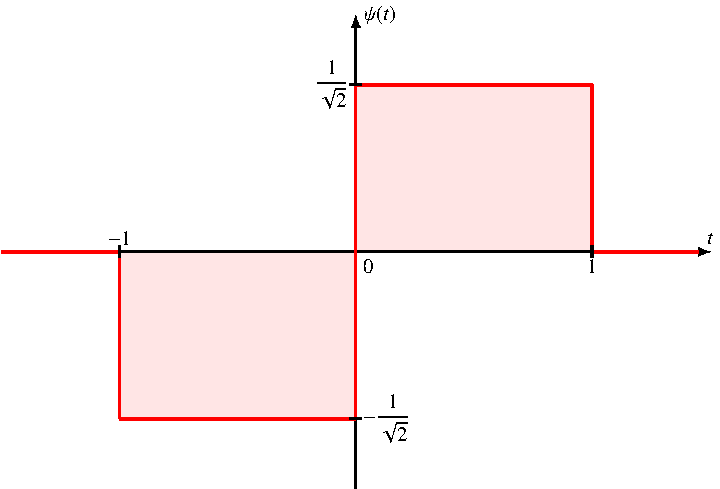
\includegraphics{chapters/4-cwt/images/psigraph.pdf}
\caption{Graph der Funktion $\psi(t)$ für das Beispiel der
Wavelet-Transformation in Abbildung~\ref{cwt:psi-cwt}.
\label{cwt:psi-graph}}
\end{figure}
\begin{figure}
\centering
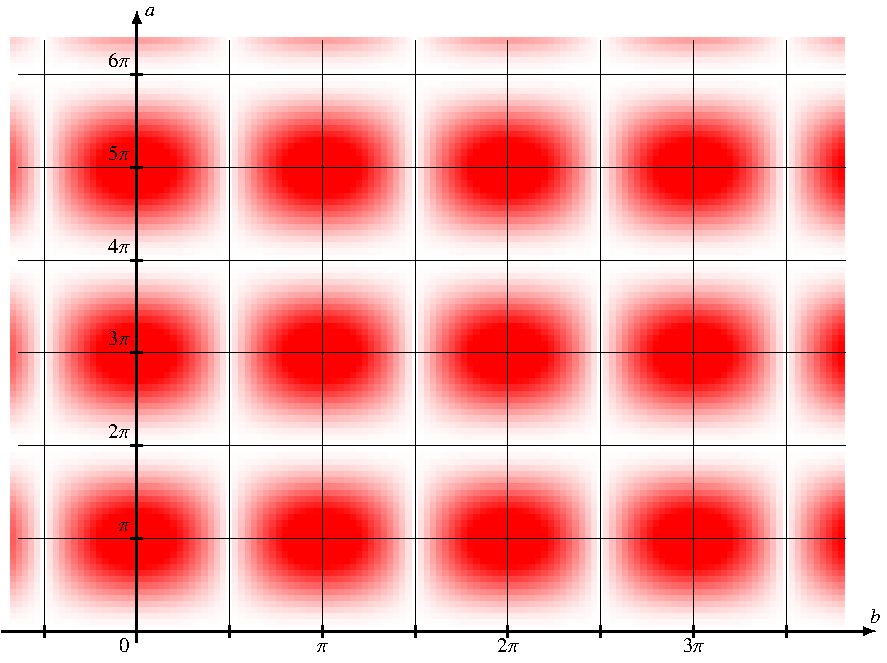
\includegraphics[width=\hsize]{chapters/4-cwt/images/psisin.pdf}
\caption{Wavelet-Transformation der Funktion $f(t)=\sin t$ berechnet
mit dem Wavelet $\psi(t)$ von Abbildung~\ref{cwt:psi-graph}
\label{cwt:psi-cwt}}
\end{figure}
Der Graph der Funktion ist auch in Abbildung~\ref{cwt:psi-graph} dargestellt.
Wir betrachten die Funktion
\[
\psi(t) = \begin{cases}
-\frac1{\sqrt{2}}&\qquad -1\le t< 0\\
\frac1{\sqrt{2}}&\qquad 0\le t< 1\\
0&\qquad\text{sonst}
\end{cases}
\]
Dies ist eine gestreckte und verschobene Version des Haar-Wavelets,
und erfüllt daher automatisch die Zulässigkeitsbedingung für ein Wavelet.
Ausserdem gilt $\|\psi\|=1$.
Gegenüber dem Haar-Mutter-Wavelet hat diese Funktion den Vorteil, dass 
sie antisymmetrisch ist, so dass auch die stetige Wavelettransformation
einer antisymmetrischen Funktion wieder symmetrisch sein wird.

Wir berechnen jetzt die stetige Wavelet-Transformat des Signals $f(t)=\sin t$.
Nach Definition ist
\begin{align*}
\mathcal{W}f(a,b)
&=
\int_{-\infty}^\infty f(t)
\frac{1}{\sqrt{|a|}}\overline{\psi\biggl(\frac{t-b}{a}\biggr)}
\,dt.
\\
\intertext{Da sich das Integral über ganz $\mathbb R$ erstreckt, können
wir das Integral um $b$ verschieben, und erhalten}
&=
\frac{1}{\sqrt{|a|}}
\int_{-\infty}^\infty f(t+b)\overline{\psi\biggl(\frac{t}{a}\biggr)}\,dt.
\\
\intertext{Substituieren wir $as=t$, können wir auch den Skalierungsfaktor
von $\psi$ auf das Signal verschieben:}
&=
\sqrt{|a|}
\int_{-\infty}^\infty f(as+b)\overline{\psi(s)}\,ds.
\\
\intertext{Für $a<0$ bekommt man ein negatives Vorzeichen, aber es tauschen
auch die Integrationsgrenzen ihre Plätze.
Jetzt können wir das Signal $f$ einsetzen und mit der Definition der
Funktion $\psi$ das Integral vereinfachen}
&=
\sqrt{\frac{|a|}{2}}
\biggl(
-
\int_{-1}^0 \sin(as+b)\,dt
+
\int_{0}^1 \sin(as+b)\,dt
\biggr)
\\
&=
\sqrt{\frac{|a|}{2}}
\biggl(
-
\biggl[-\frac{\cos(as+b)}{a}\biggr]_{-1}^0
+
\biggl[-\frac{\cos(as+b)}{a}\biggr]_{0}^1
\biggr)
\\
&=
\frac{1}{\sqrt{2|a|}}
(
\cos(b) - \cos(-a+b) -\cos(a+b)+\cos(b)
)
\\
&=
\frac{1}{\sqrt{2|a|}}
(2\cos b - \cos(b+a) - \cos(b-a))
\end{align*}
Wir betrachten einige einfach zu berechnende Werte von $\mathcal{W}f$.
Die Kosinus-Funktion ist antisymmetrisch bezüglich ungeraden Vielfachen
von $\pi/2$.
Wir setzen daher $b=(2k+1)\frac{\pi}2$ und berechnen den Wert von
\begin{align*}
\mathcal{W}f(a,b)
&=
\mathcal{W}f\biggl(a,(2k+1)\frac{\pi}2\biggr)
=
2\cos\biggl((2k+1)\frac{\pi}2\biggr)
-\cos\biggl((2k+1)\frac{\pi}2 -a\biggr)
-\cos\biggl((2k+1)\frac{\pi}2 +a\biggr)
\\
&=
0
\pm(\sin a - \sin a)
=0.
\end{align*}
Wenn $b$ ein ganzzahliges Vielfaches von $\pi$ ist, also $b=k\pi$, dann ist 
\begin{align*}
\mathcal{W}f(a,b)
&=
\frac{1}{\sqrt{2|a|}}(2\cos k\pi - \cos(k\pi +a) -\cos(k\pi-a))
\\
\intertext{Die Kosinus-Funktion ist symmetrisch bezüglich $b$, so dass die
beiden letzten Terme gleich sind.  }
&=
\frac{1}{\sqrt{2|a|}}(2\cos k\pi - 2\cos(k\pi +a))
\\
&=
\frac{1}{\sqrt{2|a|}}(2\cos k\pi - 2\cos k\pi \cos a + 2 \sin k\pi \sin a))
\\
\intertext{Der letzte Term verschwindet, weil $\sin k\pi=0$.
Im ersten Term können wir $\cos k\pi=(-1)^k$ ersetzen und erhalten}
&=
\frac{2(-1)^k}{\sqrt{2|a|}}(1 - \cos a)
\end{align*}

Die Wavelet-Transformation $\mathcal{W}f$ ist in Abbildung~\ref{cwt:psi-cwt}
dargestellt.
Intensivere Farbe bedeutet grösseren absoluten Betrag von $\mathcal{W}f$.
Immer wenn die Funktion $\psi$ so skaliert ist, dass sie auf jeder
Seite des Nullpunkts eine ganze Zahl vollständiger Sinus-Perioden abdeckt,
verschwindet der Wert der Wavelet-Transformation.
Wenn dagegen $a$ so gewählt ist, dass auf jeder Seite in halbe Periode
``übrig'' bleibt, dann nimmt die Wavelet-Transformation den grösstmöglichen
Wert an.
Da das Signal $\sin t$ periodisch ist, ist auch die Wavelet-Transformiation
$\mathcal{W}f$ periodisch in $b$.
Dies erklärt das Muster in Abbildung~\ref{cwt:psi-cwt}.
\end{beispiel}

\begin{beispiel}
\begin{figure}
\centering
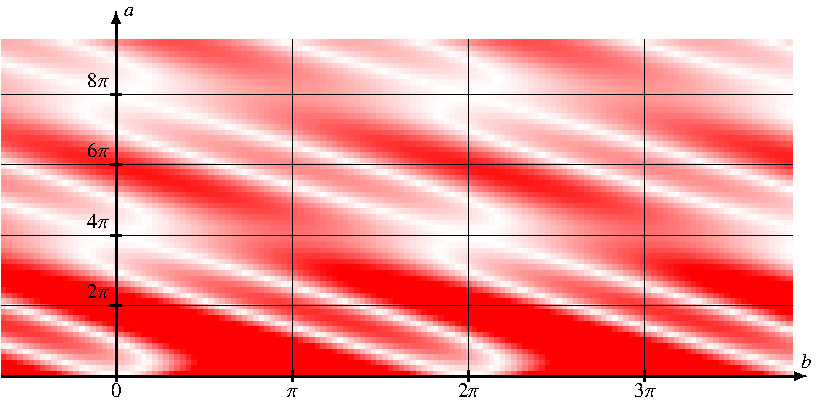
\includegraphics[width=\hsize]{chapters/4-cwt/images/wsin.pdf}
\caption{Wavelet-Transformation der Sinus-Funktion $\sin t$
mit dem Haar-Wavelet $\psi_{\text{Haar}}$
\label{cwt:wsin}}
\end{figure}
Sei wieder $\psi=\psi_{\text{Haar}}$ das Haar-Wavelet.
Wir berechnen die stetige Wavelet-Transformation der Sinus-Funktion
$f(t)=\sin t$.
Der Einfachheit halber führen wir die Berechnung der Wavelet-Transformation
zunächst für $a>0$ durch.
Nach Definition ist gilt
\begin{align*}
\mathcal{W}f (a,b)
&=
\frac{1}{\sqrt{|a|}}
\int_{-\infty}^\infty \sin t\cdot \psi\biggl(\frac{t-b}{a}\biggr)\,dt.
\\
\intertext{Da sich das Integral über die ganze reelle Achse erstreckt,
können wir $t$ durch $t+b$ ersetzen, ohne dass sich das Integral ändert.
Wir erhalten daher}
&=
\frac{1}{\sqrt{|a|}}
\int_{-\infty}^\infty \sin (t+b)\cdot \psi\biggl(\frac{t}{a}\biggr)\,dt
=
\frac{1}{\sqrt{|a|}}
\int_{-\infty}^\infty \sin (as+b)\cdot \psi(s) a\,ds.
\\
\intertext{Dabei haben wir $t=as$ substituiert.
Jetzt lässt sich das Integral explizit ausrechnen}
&=
\sqrt{a}
\int_{0}^{\frac12} \sin(as+b)\,ds
-
\sqrt{a}
\int_{\frac12}^{1} \sin(as+b)\,ds
\\
&=
\sqrt{a}
\biggl[-\frac{\cos(as+b)}{a}\biggr]_{0}^{\frac12}
-
\sqrt{a}
\biggl[-\frac{\cos(as+b)}{a}\biggr]_{\frac12}^1
=
\frac{1}{\sqrt{a}}\biggl(
-1 + 2\cos({\textstyle\frac12}a+b) - \cos(a+b)
\biggr)
\end{align*}
Die Wavelet-Transformation ist in Abbildung~\ref{cwt:wsin} als
Intensitäts-Plot dargestellt.
Je grässer $|\mathcal{W}_{\psi_{\text{Haar}}}(a,b)|$, desto intensiver
die Farbe.
Die Asymmetrie des Haar-Wavelets äaussert sich in der gegenüber 
Abbildung~\ref{cwt:psi-graph} offensichtlichen Verzerrung.
\end{beispiel}

\begin{beispiel}
Dieses Beispiel stammt aus \cite[p.~60]{buch:blatter}.
\begin{figure}
\centering
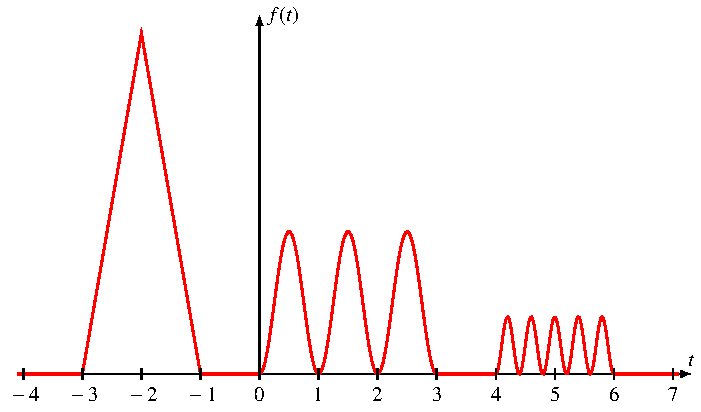
\includegraphics{chapters/4-cwt/images/f.pdf}
\caption{Funktion $f(t)$ aus \cite[p.~60]{buch:blatter}
\label{cwt:blatterfgraph}}
\end{figure}
\begin{figure}
\centering
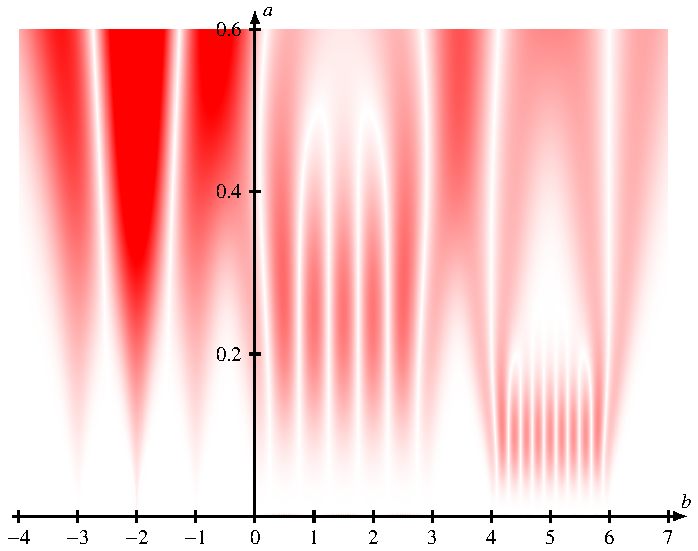
\includegraphics{chapters/4-cwt/images/notes.pdf}
\caption{Stetige Wavelet-Transformation der Funktion \eqref{cwt:blatterf}
(Graph in Abbildung~\ref{cwt:blatterfgraph}).
\label{cwt:blattercwt}}
\end{figure}
Wir berechnen die die Wavelet-Transformation der folgenden Funktion $f$
für das Mexikanerhut-Wavelet \eqref{wavelet:mexikanerhut}, wir setzen also
$\psi=\psi_M$.
\begin{equation}
f(t) = \begin{cases}
2.883 \cdot (2 - 2\,|t+2|)&\qquad -3\le t \le -1\\
1.205\cdot (1-\cos(2\pi t))&\qquad 0\le t \le 3\\
0.968\cdot \frac12(1-\cos(5\pi t))&\qquad 4\le t \le 6\\
0&\qquad\text{sonst.}
\end{cases}
\label{cwt:blatterf}
\end{equation}
Eine graphische Darstellung der Funktion ist in Abbildung~\ref{cwt:blatterf}
gegeben.
Die numerisch berechnete Transformation ist in Abbildung~\ref{cwt:blattercwt}
dargestellt.
Die Funktion besteht aus drei Teilfunktionen, die von Intervallen getrennt sind,
in denen die Funktion verschwindet.
In den Intervallen $[0,3]$ und $[4,6]$ hat die Funktion oszillatorischen
Charakter.
Die Wavelet-Transformation ist in der Lage, dieses Verhalten zu detektieren.
Es lässt sich sogar eine ungefähre Aussage über die Frequenzverhältnisse
machen.
Die Oszillation im Interval $[4,6]$ hat $2.5$-mal höhere Frequenz als im
Interval $[0,3]$, was sich darin äussert, dass die Schwerpunkte der roten
Flächen bei etwa $2.5$-mal geringerem $a$ liegen.
\end{beispiel}

In den Abbildungen \ref{cwt:psi-cwt} und \ref{cwt:blattercwt} werden 
die Skalenfaktoren $a$ auf der vertikalen Achse abgetragen.
Grössere Werte von $a$ bedeutet dabei grössere ``Wellenlänge'' des Wavelets,
so dass die ``hochfrequenten'' Koeffizienten am unteren Rand des
Intensitätsgraphen sind.
In Anwendungen der Signalverarbeitung wird daher oft $1/a$ oder $-\log a$ 
auf der vertikalen Achse aufgetragen, so dass hohe Frequenzen wie in
einem Sonogramm weiter oben dargestellt werden.

\begin{beispiel}
In diesem Beispiel verwenden wir komplexe Morlet-Wavelets
\begin{equation}
\psi(t) = e^{-\frac{t^2}2 +5it} \label{cwt:morlet}
\end{equation}
um das Sweep-Signal mit linear ansteigender Frequenz
\begin{equation}
f(t)
=
\sin(t(4+0.2t))
\label{cwt:sweep-function}
\end{equation}
zwischen $t=0$ und $t=26$.
\begin{figure}
\centering
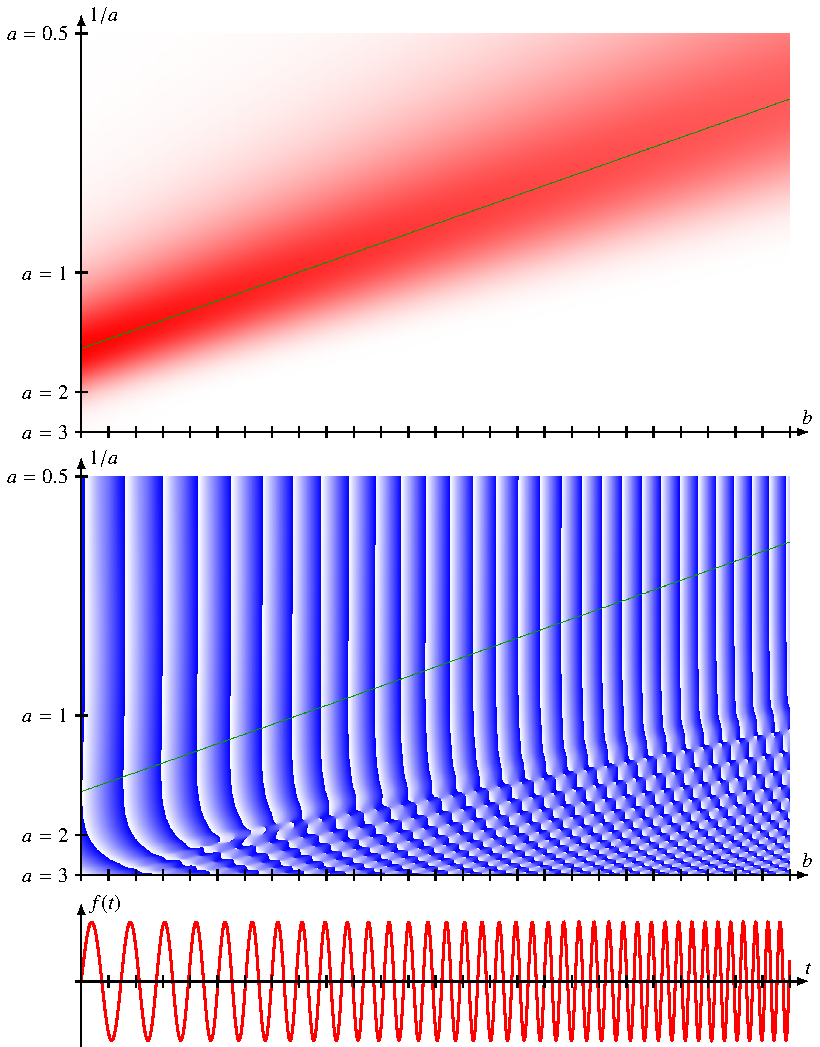
\includegraphics[width=\hsize]{chapters/4-cwt/images/sweep2.pdf}
\caption{Absolutwert und Phase der stetigen Wavelet-Transformation
der Sweep-Funktion~\eqref{cwt:sweep-function} 
für komplexe Morlet-Wavelets $\psi(t) = e^{-t^2/2+5it}$.
\label{cwt:sweep-cwt-abs-phase}}
\end{figure}
\begin{figure}
\centering
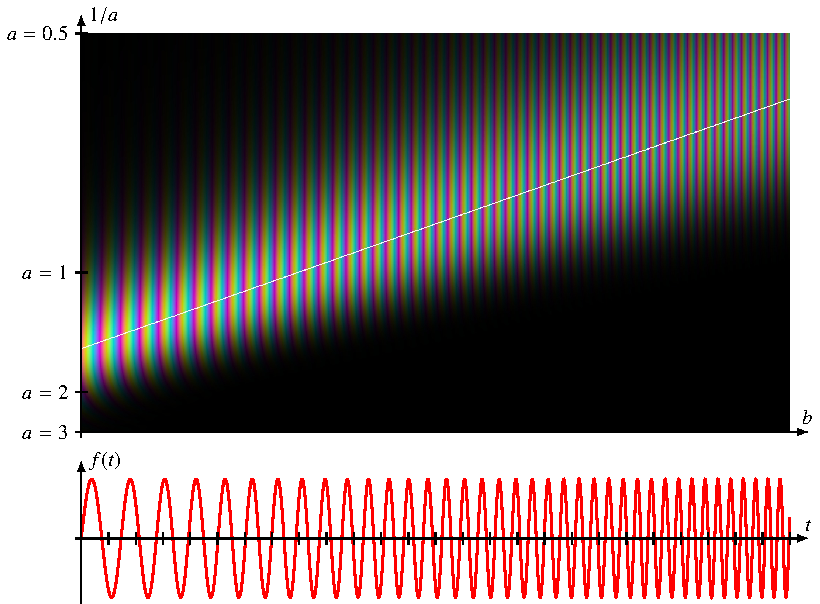
\includegraphics[width=\hsize]{chapters/4-cwt/images/sweep.pdf}
\caption{Farbcodierte Darstellung der stetigen Wavelet-Transformation
der Sweep-Funktion~\eqref{cwt:sweep-function}
für komplexe Morlet-Wavelets $\psi(t) = e^{-t^2/2} \sin(5t)$.
\label{cwt:sweep-cwt-color}}
\end{figure}
Die Resultate sind in Abbildungen~\ref{cwt:sweep-cwt-abs-phase} und
\ref{cwt:sweep-cwt-color} dargestellt.
Der Absolutwert der stetigen Wavelettransformation zeigt die aktuelle
Frequenz des Sweep-Signals an.
Das Maximum der Amplitude für jeden $b$-Wert ist in
Abbildung~\ref{cwt:sweep-cwt-abs-phase} dunkelgrün hervorgehoben.
Danke der komplexen Oszillation $e^{5it}$ ändert zwar die Phase relativ
rasch entlang des Maximums, der Absolutwert ändert dagegen nur 
langsam.
In Abbildung~\ref{cwt:sweep-cwt-color} ist die Phase durch die Farbe
codiert, auch hier wird offensichtlich, dass die Phase sehr schnell ändert,
während die Amplitude nur langsam abfällt.

Ein reelles Wavelet ergibt dagegen immer dann einen maximalen Wert der
Wavelet-Transformation, wenn die Extrema des Wavelets mit den Extrema
des Signals zusammenfallen.
Die komplexen Oszillation $e^{5it}=\cos 5t + i\sin 5t$ kann durch einen
Phasenfaktor immer so modifiziert werden, dass die Extrema des Realteils
mit den Extrema des Signals zusammenfallen.
Dieser Phasenfaktor hat genau die entgegengesetzte Phase der
Wavelettransformation.
\end{beispiel}
